Chapter \ref{cha:features} listed basic features of the ICL packages that do not pertain to image processing in the proper meaning of the word. This chapter lists and explains most image processing functionalities and interfaces.

\section{ICLUtils}

[Documentation: \iclpackageref{Utils}]\\
This ICLUtils package contains (per definition) no image processing functions, rather it provides more general classes and functions (e.g. matrix and vector classes, exceptions, debugging macros etc.).

\subsection{Matrix and Vector Classes}
Matrix and Vector algebra is very common in a lot of applications. The ICL provides two approaches for matrix and vector classes:


\subsubsection{FixedMatrix Template Class\iclclassref{FixedMatrix}{Utils}}
This class uses three template parameters \inlinecode{template<class T, unsigned int COLS, unsigned} \inlinecode{int ROWS>} to represent matrices of fixed size. FixedVectors are implemented as shallow inheriting wrappers of FixedMatrix class instances with \inlinecode{COLS=1} (\inlinecode{FixedColVector}) or \inlinecode{ROWS=1} (\inlinecode{FixedRowVector})\footnote{This cannot be implemented using typedefs, because C++ does not support templated typedefs}.
By using \emph{templated} dimension parameters, matrix dimension is fixed at compilation time, which enables the compiler to apply a lot of optimizations. Most common vector and matrix algebra functionalities \footnote{As far as I can see, actually a super-set of BLAS-level 3}, including matrix mutliplication (scalar product is just a special case here), QR-Matrix decomposition and matrix inverse and pseudo-inverse\footnote{QR-decomposition-based} implementation. \inlinecode{FixedMatrix} instances resign smart data handling to enable the compiler to apply special optimizations on fixed arrays. In particular, temporary instances (and their data) can be allocated on the stack, rather than having to allocate data on the heap.
The \inlinecode{FixedMatrix} class provides row- and column iterators, as well as extraction functions for rows, columns or rectangular sub-matrices.
Here's a concise example:
\codefile{fixed-matrix-demo-1.cpp}{Example for usage of the \inlinecode{FixedMatrix}-template class}
Please note, that \inlinecode{FixedMatrix}-pseudo inverse calculation is out-sourced to a dedicated header \iclheaderref{Utils}{FixedMatrixUtils} to reduce complexity of the FixedMatrix header file.

\subsubsection{DynMatrix Template Class\iclclassref{DynMatrix}{Utils}}

In contrast to the \inlinecode{FixedMatrix} template class, the \inlinecode{DynMatrix} template class uses a single template parameter which defines the actual datatype of the matrix elements. Matrix dimensions are dynamic at runtime, which enables us to provide e.g. a \inlinecode{setBounds} member function. In addition, \inlinecode{DynMatrix} instances can be assigned with \inlinecode{DynMatrix} instances of another size. Dynamic sized data types need dynamic data handling\footnote{using \inlinecode{new []} and \inlinecode{delete []}}. This besides allows a more flexible mechanism: optional shallow data wrapping. \inlinecode{DynMatrix} instances can be set up to handle their data autonomously (using \inlinecode{new []} in the constructor and \inlinecode{delete []} in the destructor), or to \emph{count on} external data handling. Most other functionalities such as matrix multiplication or matrix inverse are also available here. Actually, matrix inverse in the \inlinecode{FixedMatrix} class is implemented by a shallow wrapping \inlinecode{DynMatrix} function call.\\
In addition to the actual \inlinecode{DynMatrix}-class, we provide another header file that is called \iclheaderref{Utils}{DynMatrixUtils}. This contains a large set of arithmetical functions in different calling manners (source-destination, source-only). Additionally \inlinecode{add}, \inlinecode{sub} and \inlinecode{mult} are provided multiple times to allow e.g. multiplication of two matrices A and B as $A^{\tau}B$ without the need to transpose A explicitly before.\\[10pt]
The \inlinecode{DynMatrix}-template class is very tightly integrated with the  \inlinecode{Img<T>}-template class. The index operator (\inlinecode{Img<T>::operator[](int channel)} returns an instance of \inlinecode{DynMatrix<T>} that wraps the images channel data shallowly. This enables the programmer switch between image- and matrix notation very easily. Besides \inlinecode{Img<T>} instances can be created as shallow wrappers of a set of \inlinecode{DynMatrix<T>}-instances (one \inlinecode{DynMatrix<T>}-instances corresponds to one image channel) by using an appropriate \inlinecode{Img<T>}-constructor, that takes up to 5 \inlinecode{DynMatrix<T>}-arguments.\\
This also allows the user to apply arbitrary image processing functions on \inlinecode{DynMatrix<T>} instances.




\subsection{Time and Timing classes}
ICL provides some time and timer classes to facilitate handling of time values and frame rates:
\begin{itemize}
\item The \inlinecode{Time} class (\iclclassref{Utils}{Time}) is the basis for timing classes. It provides a static function \inlinecode{now()} to obtain the current system time, as well as a variety manipulation and conversion functions.
\item The \inlinecode{Timer} (\iclclassref{Utils}{Timer}) class allows to compute time differences e.g. for benchmarking.
\item The \inlinecode{StackTimer} (\iclclassref{Utils}{StackTimer}) can be used with the macro \inlinecode{BENCHMARK\_THIS\_FUNCTION} to profile a function.
\item \inlinecode{FPSEstimator} (\iclclassref{Utils}{FPSEstimator}) and \inlinecode{FPSLimiter} (\iclclassref{Utils}{FPSLimiter}) can be used to compute or to limit the FPS\footnote{Frames Per Second} count of a application.
\end{itemize}

\subsection{Threading Classes}
The \inlinecode{Thread}-class (\iclclassref{Utils}{Thread}) and the \inlinecode{Mutex}-class (\iclclassref{Utils}{Mutex}) are simple object-oriented wrappers for the pthread library.

\subsection{ProgArg-Environment} 
As a lot of applications need to parse command line parameters, ICL provides a simple interface to define, explain, extract and parse command line arguments (\iclheaderref{Utils}{ProgArg}). Application arguments are always fixed and need to be accessible globally, so the program argument environment is  implemented as a set of global functions each having the \inlinecode{pa_}-prefix. \inlinecode{pa\_init()} can be used to define the list of allowed program arguments and their specific count of sub-arguments\footnote{E.g consider a program argument \inlinecode{-size} could be implemented with a single sub-argument: the size.}. \inlinecode{pa\_exmplain()} explains sub-arguments. \inlinecode{pa\_defined()} and \inlinecode{pa\_arg()} are used to obtain information of the actual given program arguments.  The \inlinecode{pa\_subarg()} template function can be used to extract and parse given sub-arguments e.g. as \inlinecode{int}:
\displaycode{int c = pa\_subarg<int>("-channels",0,3);}
or as \inlinecode{std::string}
\displaycode{Size size = translateSize(pa\_subarg<std::string>("-size",0,"VGA"));}. More information can be found in the documentation.

\subsection{Utility Structures}
Firstly, there are 3 main utility structures:
\begin{enumerate}
\item The \inlinecode{Size}-class (\iclclassref{Core}{Size}), which in substance consists of an \inlinecode{int}-width and -height parameter, represents e.g. image-, widget-, ROI,  or screen sizes.
\item The \inlinecode{Point}-class (\iclclassref{Core}{Point} ; and it's \inlinecode{float}-precision variation \inlinecode{Point32f}; \iclclassref{Core}{Point32f}), should be used to defined 2D-locations e.g. pixel locations, ROI-offsets or perhaps region-centers.
\item At last, the \inlinecode{Rect}-class (\iclclassref{Core}{Rect}; also available with floating point precision; \iclclassref{Core}{Rect32f}) with essentially combines a \inlinecode{Point} and a \inlinecode{Size} to represent rectangular regions, bounding-boxes, ROI's etc.
\end{enumerate}
All these classes are derived from corresponding IPP data types (\inlinecode{ippPoint}, \inlinecode{ippSize} and \inlinecode{ippRect}) in case of having IPP support, which enables the programmer to pass e.g. an \inlinecode{icl::Point} directly to an IPP-function.

\subsubsection{Lines}
The \inlinecode{Line} and \inlinecode{Line32f} classes (\iclclassref{Core}{Line}, and \iclclassref{Core}{Line32f}). Are provided not only as an interface for representing 2D-Lines given by two points. In actual fact, they provide an efficient mechanism to sample lines into an image grid using Bresenham's line algorithm\footnote{See \hrefn{http://de.wikipedia.org/wiki/Bresenham-Algorithmus}}.

\subsubsection{Ranges}
At last, there's a template class representing ranges: \iclstructref{Core}{Range} and it's extension \iclstructref{Core}{SteppingRange}.

\subsection{String-Utilities}
To facilitate string processing (which is still a bit complicated in C++), the header \iclheaderref{Utils}{StringUtils} is provided in the ICLUtils package. It contains functions to parse \inlinecode{std::strings} into given data types (template based, \inlinecode{T parse<T>(const std::string&)} and to convert given data-types into strings (\inlinecode{std::string str(const T&)}). Furthermore, there are variants of these functions, that work on \inlinecode{std::vector} instances to convert or parse ranges at once.\\
Moreover, ICL provides conversion functions to translate sizes, formats, depths etc. into strings and back. These functions are located in the \iclheaderref{Utils}{Utils} and their names are \inlinecode{translateSize}, \inlinecode{translateFormat} etc.

\subsection{Types}
Types and enumerations have been presented and discussed in section \ref{sec:typedef-confusions}. Types are declared in \iclheaderref{Utils}{BasicTypes}.

\subsection{XML-Parser}
To be able to use xml-data and configuration files without getting an extra software-dependency, ICL uses it's own simple XML-Parser. This of course entails some issues on the complexity of XML-files, that can be parsed. Actually, some features (like namespaces or XML-schematics) are just not supported at all.\\
However, the XML-Parser works well for our purpose: It can be used to easily parse XML-documents or to query and filter nodes from the Documents tree structure. Furthermore, we use it successfully to create and to parse instances of the \inlinecode{ConfigFile} class, that provides high convenience for using configuration files in applications (See \ref{subsec:config-file})

\subsection{Configuration Files\label{subsec:config-file}}
The \iclclassref{Utils}{ConfigFile}-class can be used to facility handling of dynamic configurable applications. Of course, one can make heavily use of program arguments, however this makes is difficult to save parameters or to distribute configuration parameters via revision control systems like e.g. subversion\footnote{\hrefn{http://de.wikipedia.org/wiki/Subversion\_(Software)}}. \inlinecode{ConfigFile} instances can be created very easily in the C++ source code, and their contents can be obtains very simply. Most of the time, a simple one-line statement is sufficient to get a certain entry at runtime. On the other side, the configuration file itself uses a simple XML-subset which facilitates both, parsing of the document as well as referencing entries non-ambiguously. Here's a tiny example:

\codefile{config.xml}{config.xml}

Corresponding source file:

\codefile{config-file.cpp}{ConfigFile use case}

And resulting configuration file:

\codefile{other.xml}{Written configuration file other.xml}

\subsection{ConfigEntry Utility class}
The \inlinecode{ConfigEntry}-template class \iclclassref{Qt}{ConfigEntry} provides a convenient access to data entries of a ConfigFile instance. \inlinecode{ConfigEntry} instances are always \emph{templated} to their actual type: e.g. \inlinecode{ConfigEntry<int>} or \inlinecode{ConfigEntry<float>}. \inlinecode{ConfigEntry} objects can be instantiated with a given key-value (which is the '.'-separated path to the referenced ConfigFile element), a default value (which is used, if the given key was not found) and the referenced ConfigFile (which is the singleton static ConfigFile instance by default). Furthermore, \inlinecode{ConfigEntry}-instances can simply be used in the same way as their template parameter type, because they provide an implicit cast-operator for this type.\\
Using ConfigEntry instances is useful if your application also uses the \inlinecode{ConfigFileGUI} utility class \iclclassref{Qt}{ConfigFileGUI} which is presented in \ref{subsec:configfile-gui}.\\
In addition, the header \iclheaderref{Qt}{ConfigEntry} provides some convenience macros to create local instances of the \iclclassref{ConfigEntry} class.

\section{ICLCore}

[Documentation: \iclpackageref{Core}]\\
The Core-package contains, apart from the image base class \inlinecode{ImgBase} and template classes \inlinecode{Img<T>}, fundamental image processing functions and utility classes. In particular, it contains the header \iclheaderref{Core}{Types}, that declares most common ICL data types and enumerations. Furthermore, there are mathematic functions, random number generators, utility functions for converting and copying images and some utility structures like rectangles, points and lines.

\subsection{Image classes}
The image classes have been described in detail in chapter \ref{cha:img-base-functions} and \ref{cha:img-class-functions}.


\subsection{Mathematic Functions}
Also some fundamental mathematic functionalities are provided in the package. The header \iclheaderref{Core}{Mathematics} contains some stochastic utility template functions for computation of mean, variance and standard derivation of a range. Also color-histogram calculating functions (\inlinecode{hist} and \inlinecode{channelHisto}) are available by including this header. More information can be obtained from the header documentation (mentioned above).

\subsection{Random Number Generators}
Formerly a part of the header \iclheaderref{Core}{Mathematics}-header, random number generators are not provided by the header \iclheaderref{Core}{Random}. Actually, only two different distributions are currently supported: uniform- and gaussian distribution. However a set of functions are provided for each distribution to facilitate random number (and random range) generation. \\
Firstly, there's an overloaded \inlinecode{randomSeed()} function, that can be used to initialize the systems random generator engine, with an optinal \emph{seed-value}. If no seed value is given, current system time is used for initialization. Furthermore, a class called \inlinecode{RandomSeeder} (\iclstructref{Core}{RandomSeeder}) is provided which can be instantiated on some stack to force random number generation engine initialization at program startup. \\
In Addition, there's a set of initializer functors (\iclclassref{Core}{URand},\iclclassref{Core}{URandI},\iclclassref{Core}{GRand} and \iclclassref{Core}{GRandClip}), that can be used e.g. with \inlinecode{std::fill} to initialize range elements randomly. 



\section{ICLCC\label{sec:cc}}

[Documentation: \iclpackageref{CC}]\\
The \textbf{C}olor \textbf{C}conversion package provides a powerful environment for converting images color formats. Additionally data layout conversion functions (\inlinecode{interleavedToPlanar} and \inlinecode{planarToInterleaved} are implemented in this package (available by including the \iclheaderref{CC}{CC}-header) and a powerful \inlinecode{Converter}-class (\iclclassref{CC}{Converter}), that allows convert images with different sizes, formats and depths\footnote{or even all at once} into each other while preserving image content.


\subsection{Color Conversion}

As illustrated in section \ref{sec:image-features} ICL images possess a \inlinecode{format} parameter that defines the images actual color format (e.g. RGB HLS or gray). As most algorithms process images regardless their color formats, color conversion was outsourced into the dedicated \iclpackageref{CC}-package. Basically, all color conversion algorithms are implemented with a single function called \inlinecode{cc} (also available in the \iclheaderref{CC}{CC}-header. \inlinecode{cc} is able to convert pixels from a source image into a given destination image. Source and destination color formats are extracted automatically from the given images. Optionally, \inlinecode{cc} can be setup to process an images ROI only.\\
Base format for color conversion is the \emph{sRGB}\footnote{\hrefn{http://en.wikipedia.org/wiki/SRGB}} format (represented by the \inlinecode{format}-enum value \inlinecode{formatRGB}). All other formats can be converted \emph{from} and \emph{into} the sRGB-format natively. Some other \emph{cross-conversions} are implemented by first converting source image pixels into sRGB, before conversion from sRGB into the desired destination format is available. The \iclheaderref{CC}{CC}-header provides a good overview of the implemented formats and their conversion performance.\\
If color conversion performance is not fast enough, it can be optimized using a lookup table, that can be created on automatically on demand by calling the \inlinecode{createLUT} function.\\
By the way, the color conversion function \inlinecode{cc} is implemented using massive template-expansion. This enables \inlinecode{cc} to perform a \inlinecode{depth}-conversion simultaneously (by the way, this is why \inlinecode{iclCC.cpp} needs that much time to compile).

\subsection{General Parameter Conversion}

If also an images size must be adapted, there's need for some temporary buffers. The \inlinecode{Converter} (\iclclassref{CC}{Converter}) class automatically handles internal buffers for \inlinecode{depth}-, \inlinecode{size}- and \inlinecode{format}-conversion. Furthermore it provides the ability to select the order of different conversion steps.
 

 
\subsection{Data Layout Conversion}

As motivated in chapter \ref{cha:what-is-the-icl}, ICL's images do always use planar data layout, however sometimes available image data is interleaved, or ICL-image data must be converted into interleaved data layout. The \iclheaderref{CC}{CC}-header also provides two conversion functions for this tasks: \displaycode{interleavedToPlanar}
\displaycode{planarToInterleaved}

Both functions are highly optimized and -- if supported -- IPP accelerated. Additionally, both functions are able to apply a \inlinecode{depth}-conversion too, and the provide source and destination ROI support. As there's no interleaved image format in the ICL, interleaved image data is always just represented by a single data pointer; the interleaved images ROI is determined from the given \inlinecode{lineStep} argument.





\section{ICLIO\label{sec:io}}

[Documentation: \iclpackageref{IO}]\\

The IO-package provides functions and classes for reading and writing image from- and to different devices. The most common interface is the \inlinecode{Grabber} (\iclclassref{IO}{Grabber}). All image input devices are implemented as specializations of this \inlinecode{Grabber}-class, which provides a generic interface for grabbing images and setting camera parameters and capture modes (see section \ref{sec:grabber-feature-adjustment}). Currently, the following grabbers are available:

\begin{enumerate}
\item \inlinecode{FileGrabber} [\iclclassref{IO}{FileGrabber}]:\\
 For reading image files in most different formats. .ppm, .pnm and .pgm as well as a special icl-format \emph{.icl} are implemented natively without any external software dependencies. .jpeg-files can be read with a wrapper of libjpeg. All other file-formats are passed to an libImageMagic++\footnote{\hrefn{http://www.imagemagick.org/Magick++/}}-wrapper (currently this supports about 100 more or less common file formats)
%
\item \inlinecode{DCGrabber} [\iclclassref{IO}{DCGrabber}]:\\
The \inlinecode{DCGrabber} grabs images from fire-wire aka IEEE-1394 camera devices. Basically it wraps the libdc1394 library\footnote{\hrefn{http://sourceforge.net/projects/libdc1394/}} for accessing cameras, that meet the IIDC DCAM standart\footnote{\hrefn{http://de.wikipedia.org/wiki/DCAM}}, and which gave the grabber it's name. DC-Camera features, image acquisition modes and framerates are made accessible via the Grabbers feature \emph{setter}- and \emph{getter}-functions.
%
\item \inlinecode{PWCGrabber} [\iclclassref{IO}{PWCGrabber}]:\\
The \textbf{P}hillips \textbf{W}eb\textbf{C}am grabber can be used to grab images from cameras that use the linux pwc kernel module\footnote{\hrefn{http://www.saillard.org/linux/pwc/}}.
\item \inlinecode{UnicapGrabber} [\iclclassref{IO}{UnicapGrabber}]:\\
This grabber wraps the \textbf{unicap}-library\footnote{\hrefn{http://unicap-imaging.org/}} which provides a generalized access to fire-wire as well as video-4-linux/video-4-linux-2 devices.  
\item \inlinecode{VideoGrabber} [\iclclassref{IO}{VideoGrabber}]:\\
This grabber implementation uses libxine\footnote{\hrefn{http://www.xine-project.org}} to use video files as image data source. The VideoGrabber provides functions to adjust video playback speed (by default, videos are grabbed frame by frame, but not faster then the actual movie framerate). Furthermore, if video playback speed is close to the movie framerate, the VideoGrabber will also playback sound. 
\item \inlinecode{SwissRangerGrabber} [\iclclassref{IO}{SwissRangerGrabber}]:\\
The SwissRanger is a so-called time-of-flight camera from the Mesa-Imaging company\footnote{\hrefn{http://www.mesa-imaging.ch}}. It uses a set of pulsed IR-LED's to compute depth images. This grabber uses the libmesasr-library for accessing camera features and image data. The SwissRanger camera also provides gray-scale images and a confidence map, which tells the user the estimated accuracy for each depth-pixel.
\item \inlinecode{DemoGrabber} [\iclclassref{IO}{DemoGrabber}]:\\
This is just a tiny utility class, which can be used e.g. to test an application if no appropriate source device is currently available. It creates images with a small moving red rectangle.
\item \inlinecode{XCFPublisherGrabber} [\iclclassref{IO}{XCFPublisherGrabber}]:\\
This grabber utilizes the XCF-framework to receive images via network. Images can e.g. be send from other applications using the \inlinecode{XCFPublisher} class (\iclclassref{IO}{XCFPublisher} or the demo application \inlinecode{icl-xcf-publisher}.
\item \inlinecode{XCFMemoryGrabber} [\iclclassref{IO}{XCFMemoryGrabber}]:\\
Here also XCF is used, but now in combination with the ActiveMemory which is an XML-based active blackbord for interprocess communication. 
\item \inlinecode{XCFServerGrabber} [\iclclassref{IO}{XCFServerGrabber}]:\\
This is the 3rd implementation of an XCF-based grabber. This grabber utilized XCF's remote method invocation concept for grabbing images from an image server.
\item \inlinecode{GenericGrabber} [\iclclassref{IO}{GenericGrabber}]: \textbf{This is the grabber that should be used by your application!}\\
The \inlinecode{GenericGrabber} internally wraps one of the other grabbers. Which actual \inlinecode{Grabber}-instance is used internally depends on a string values, which is passed to the \inlinecode{GenericGrabber}-constructor. This enables the programmer to create applications, that are able to work with most different input devices. Using the \inlinecode{GenericGrabber} instead of some other Grabber instances directly provides a lot of advantages:
\begin{itemize}
\item Applications that use a generic grabber can simple be set up to use any input device
\item In particular, one can easily switch from a camera device to stored image files
\item The compilation procedure of applications doesn't have to check for a particular Grabber/library to be present or something
\item There's only a single additional pointer access for this improved flexibility
\end{itemize}
The \inlinecode{GenericGrabber} constructor gets two arguments. The first argument is one (or a comma-separated list) of \inlinecode{pwc}, \inlinecode{unicap}, \inlinecode{dc}, \inlinecode{file} or  \inlinecode{demoe} and determines the grabber type. If a list if given, it is searched successively for a supported device type. The second argument is also of type \inlinecode{std::string} and provides additional information for the creation of the internal Grabber instance. As each Grabber needs other constructor parameters, this argument's syntax depends on the first argument as well. To allow to specify also arguments to a list of possible device types, the device type is also given here again. Some examples will explain this in detail:
\begin{itemize}
\item \inlinecode{GenericGrabber("pwc","pwc=0")}: Creates a \inlinecode{GenericGrabber} instance that wraps a \inlinecode{PWCGrabber} for \texttt{/dev/video0}
\item \inlinecode{GenericGrabber("pwc,file","pwc=0,file=*.ppm")}: As above, but with file grabber fallback
\item \inlinecode{GenericGrabber("file","file=images/*.ppm")}: \inlinecode{FileGrabber} that uses all files in \texttt{./images} with suffix \texttt{.ppm}
\item \inlinecode{GenericGrabber("dc","1")}: internally a \inlinecode{DCGrabber} is wrapped, that uses DC-device index 1 (available devices are enumerated internally)
\item \inlinecode{GenericGrabber("unicap","*Phillips*")}: Use the first unicap device, which matches the given string pattern
\item \inlinecode{GenericGrabber("pwc,file,dc","pwc=0,file=images/*.ppm,dc=1")}: An example combination
\end{itemize}
In most applications, the actual Grabber, that should be used is determined by a progarg-argument (See \iclheaderref{Utils}{ProgArg}). To enhance convenience for instantiation of  \inlinecode{GenericGrabber}s using progarg input, a special macro \inlinecode{FROM\_PROGARG} is provided. The following example illustrates how to use this macro. 
\codefile{generic-grabber-from-progarg.cpp}{Creation of a \inlinecode{GenericGrabber} instance from a programm argument}

Now, the resulting application (we call it \inlinecode{app} here) can be run e.g. with \inlinecode{app -input dc 0} to use \inlinecode{DCGrabber} input. or with \inlinecode{app -input file images/*.ppm} to use image files as input.\\ \textbf{Please note} that the progarg-name \inlinecode{-input} is ICL's default for selection of an application's input device. Applications should not break with this conventions, unless, there are more than one input devices that must be specified somehow else (e.g. with \inlinecode{-left} and \inlinecode{-right} resp.)


\end{enumerate}


\subsection{What is the best Grabber for Fire-Wire devices?}
Unicap is partially redundant to the \inlinecode{DCGrabber} class, however both interfaces are completely independent. Grabbing from Fire-wire devices runs a little bit faster with the \inlinecode{DCGrabber}-class. The \inlinecode{DCGrabber} class is optimized to provides images with a minimal latency and is a bitter better here. 

\subsection{Feature Adjustment\label{sec:grabber-feature-adjustment}}
The \inlinecode{Grabber}-interface \iclclassref{IO}{Grabber} defines not only the way, how images can be obtained from \inlinecode{Grabber}-implementations, but also how grabber parameters or properties can be got and set. All grabbers have a special list of properties, which can be obtained by the \inlinecode{getPropertyList}-function. This function must be implemented by all classes that are derived from the \inlinecode{Grabber} class. It returns an \inlinecode{std::vector<std::string>} that contains the \textbf{names} of the supported properties. Each property has a so-called \emph{type}, that is defined by the grabber too (the type of a property is returned by the \inlinecode{getType(propertyName)} function. The type of the property defines how possible property value are defined. Possible types are:
\begin{itemize}
\item \textbf{range}\\In this case the property may have values within a defined float range (sometimes with a given fixed stepping between valid values). In a GUI , one might just use a slider to adjust such properties.
\item \textbf{value-list}\\In this case the properties possible values are defined by a list of possible float values. GUI's will probably use a combo-box containing possible float values for this kind of property.
\item \textbf{menu}\\Here, also a list defines allowed values, but here, values are strings. Again, such properties can best be adapted interactively by using a combo-box GUI element.
\item \textbf{command}\\This is a very special property type. Commands have no values at all. A command is e.g. used to make PWC-based camera save it's current parameters to the permanent camera memory. A GUI will provide commands maybe using a push-button component.
\item \textbf{info}\\ Info properties are read-only, so info-properties can't be set from externally.
\end{itemize}
Having estimated which type a certain property has (using the \inlinecode{getType(propertyName)} method in the Grabber class), the property value can be got/set using \inlinecode{getValue} and \inlinecode{setValue} respectively. 

\subsection{Desired Parameters}
The \inlinecode{Grabber}-interface \iclclassref{IO}{Grabber} also provides functions that handle the Grabbers desired parameters. To explain this one must understand, that there are always two different kinds of image parameters:
\begin{itemize}
\item The image parameters, that result from the current settings of the input device. E.g. a firewire camera might provide an image acquisition mode with VGA resolution and RGB color format or (to save bandwidth of the firewire interface) also another VGA-mode where images are YUV-411-encoded. We call this image parameter set the \emph{device-parameters}.
\item In addition there is another kind of parameters, which we call the \emph{desired parameters}. This parameters describe the size, format, etc. of images that are produced by the \inlinecode{Grabber}-instance. All Grabbers will ensure, that new images have exactly this desired format unless a special flag is set (function \inlinecode{setIgnoreDesiredParams}). \textbf{Note:} In general device parameters are not adapted to simplify creation of an appropriate new image, but the image in device-parameters is converted into the desired parameters.
\end{itemize}
We decided to have this two parameter sets to make grabber instances abstract from the underlying device, however there are situations where it is useful to be able to deactivate this mechanism: E.g. if one uses a \inlinecode{FileGrabber} instance, he might want to read the images in the real size, or when obtaining images via network (\inlinecode{XCFPublisherGrabber}). Most of the time camera grabbers provide RGB images when the ignore-desired-params flag is set to true.

\subsection{Using Grabbers}

The essential class of the IO package is the \inlinecode{Grabber}-class. Here's a short example of how to use a Grabber

\codefile{using-a-grabber.cpp}{Simple use of a \inlinecode{Grabber}-instance}

As one can see, the essential function to grab the next image from a \inlinecode{Grabber} instance is called \inlinecode{grab}. The \inlinecode{grab(..)} can be called  in two different ways: If no parameter of type \inlinecode{ImgBase**} is given, the grabber internally handles a buffer image, which is adapted to appropriate parameters and returned as \inlinecode{const ImgBase*} (\inlinecode{const} to emphasise that the \inlinecode{Grabber} instance owns this image. Grabbers ensure, that this image is valid and not changed until the next call to the \inlinecode{grab()}-function or of course until the Grabber instance is released. If one wants to have read/write access to a grabbed image he has several options:

\begin{itemize}
\item The first option is to pass an \inlinecode{ImgBase**} to the grab function. In this case the grabber will adapt the referenced image parameters or -- if the given \inlinecode{ImgBase**} points to a NULL-\inlinecode{ImgBase*} -- even create it. \textbf{Note:} That some grabbers do not support this feature, however, this is the most accurate version that has also an optimal performace.
\item Another option is to copy the obtained image using the \inlinecode{ImgBase}-function \inlinecode{deepCopy}. This function returns a new \inlinecode{ImgBase*} which has to be deleted lateron.
\item If the user wants to have direct access to the image pixels, he has check the actual image depth. This can be bypassed by using the \inlinecode{ImgBase}-function template \inlinecode{convert}.
\item However sometimes if one know what he's doing it might be possible just to remove the const-ness from the obtained image by using the \inlinecode{const\_cast}-operator of C++.
\end{itemize} 

The following example demonstrates how to access pixels from a recently grabbed image.

\codefile{using-grabbed-images.cpp}{How to access pixels of grabbed images}

\subsection{File class}
The \inlinecode{File}-class \iclclassref{IO}{File} is a simple File implementation, that provides functions to read or to write files, or to check whether a given file exists. Furthermore, the \inlinecode{File} class is able to handle zipped files if the ICL was compiled with zlib support.


\section{ICLBlob\label{sec:blob}}

[Documentation: \iclpackageref{Blob}]\\

The package \iclpackageref{Blob} provides functions for blob-detection/tracking. The most common class of the package is the \inlinecode{RegionDetector}  (see \iclclassref{Blob}{RegionDetector}), which performs a fast connected components analysis on images. The package subsumes different approaches for blob detection, which are presented in the following subsection.

\subsection{What is a \emph{Blob}}
Here, a \emph{Blob} is a set of connected pixels, that have to fulfill a certain criterion of homogeneity (e.g. all pixels have exactly the same value, or all pixels euclidian color distance to a reference color is below a certain threshold). The term of \emph{connection} must also be defined more exactly, to avoid misunderstandings: We assume pixels to be connected to all pixels in its neighborhood, which in turn is given by the 4 pixels (to the left, to the right, above and below) next to the reference pixel. 
Even though an also very common neighborhood defined by the 8 nearest pixels to a reference pixel is often used, we resign of it because of its higher computational complexity. 

\subsection{Color based Blob detection}
The first part of the \iclpackageref{Blob}-package is the Color based Blob detection framework, which essentially consists of the classes \iclclassref{Blob}{ColorBlobSearcher}, \iclclassref{Blob}{DefaultColorBlobSearcher}, \iclclassref{Blob}{FoundBlob}, \iclclassref{Blob}{PixelRating} and \iclclassref{Blob}{PixelRatingGroup}. Introducing documentation can be found in the reference of the \iclclassref{Blob}{ColorBlobSearcher} class.\\
Within the color based blob detection framework, blobs are detected globally, so different blobs must have different colors.

\subsection{Region detection / connected component analysis}
Here, the \iclclassref{Blob}{RegionDetector} is the main class. The Region detector performs a fast connected component analysis on images and provides a list of all connected regions in an image (again using the 4-pixel neighbourhood). The \inlinecode{Region} (see \iclclassref{Blob}{Region}) provides many function to compute region features like the center of gravity, the boundary or even local PCA\footnote{Principal Component Analysis (google)} information. Internally, the \inlinecode{RegionDetector} uses an intermediate representation of \inlinecode{Region}s: a list of so called \emph{scan lines}. These scan lines are horizontal image lines with a single identical gray value. Furthermore, they can efficiently be stored by a tuple $(x_{start},x_{end},y,value)$ and most region features can be calculated very efficiently on this lines (in comparison to calculate features on the image pixels). Currently there's no possibility to define certain criterions of homogeneity, than the most simple one which is currently used: all pixels within a certain region must have an identical gray value. 

\subsubsection{SimpleBlobSearcher}

On top of the \inlinecode{RegionDetector} class there's a higher level wrapper for detection of colored blobs in images: the \inlinecode{SimpleBlobSearcher} (see \iclclassref{Blob}{SimpleBlobSearcher}). This class is well documented and shall not be explained here in detail. However, it's nice to know, that the \inlinecode{SimpleBlobSearcher} provides a very simple interface for a reference-color/threshold based detection of multiple blobs in an image.

\subsection{Blob-Tracking}

In comparison to blob detection, \emph{blob tracking} means to track blobs/regions successively through time. Here, the ICL currently provides two different approaches: 
\begin{itemize}
\item A simple MeanShiftTracker implementation (see \iclclassref{Blob}{MeanShiftTracker}). The mean-shift algorithm is a very common algorithm in computer vision, which is well-discussed and well interpreted in literature. Our implementation uses the basic mean shift algorithm rather than one of its various extensions.
\item A generic yet powerful layered approach which's basic idea was also patented somewhere from somewhere else\footnote{we found that out later}. However, our tracking assignment mechanism better. The most common class is the \inlinecode{PositionTracker} (see \iclclassref{Blob}{PositionTracker}) and the \inlinecode{VectorTracker} (see \iclclassref{Blob}{VectorTracker}). For more details start reading here: \iclclassref{Blob}{PositionTracker}.
\end{itemize}


\section{ICLFilter}

[Documentation: \iclpackageref{Filter}]\\

The ICLFilter package provides a large variety of image filtering classes. When talking about image filters some misapprehensions can arise. To prevent this, the following sub-section will shortly introduce our understanding of image filters.

\subsection{Our Definition of Image \emph{Filters}}

In a most general view on image filters, a filter can be seen as a kind of black box that has N image inputs and M image outputs. However this view brings us a very generic interface for image filters which is most of the time not very feasible. \\
Most common filters (e.g. binary image operations, linear filters or neighborhood operations) only need a single input and output image. Another larger group of filters subsumes filters that get exactly two input images and that have only a single output image (e.g. arithmetical/logical per-pixel image operations or image comparison filters).
To avoid a large computational overhead arising of a too general interface, we currently support two dedicated filtering interfaces for the above mentioned 1-1 and 2-1 input-output combinations. To obviate further misunderstandings, we call this filter groups \emph{unary operations} and \emph{binary operations} respectively (represented by the C++-interfaces \iclclassref{Filter}{UnaryOp} and \iclclassref{Filter}{BinaryOp}).

For a better overview, the ICLFilter package documentation is grouped into the following modules:

\begin{enumerate}
\item Unary operations [\ref{subsec:unary-ops}]
\item Binary operations [\ref{subsec:binary-ops}]
\item Affine operations (also unary) [\ref{subsec:affine-ops}]
\item Neighbourhood operations (also unary) [\ref{subsec:nbh-ops}]
\item In-place operations [\ref{subsec:inplace-ops}] 
\item Other operations [\ref{subsec:other-ops}]
\end{enumerate}


\subsection{Unary Operations\label{subsec:unary-ops}}
Actually, most implemented operations have this type. All implementations in this group implement the \inlinecode{UnaryOp}-interface (see \iclclassref{Filter}{UnaryOp}). Unary operations implement a 1-1 input/output relation which entails, that unary operations cannot be used to apply in-place operations on images\footnote{see subsection \ref{subsec:inplace-ops} for this kind of operations}. Unary operations \emph{always} use two different images: an input image and an output image. If you want to apply a unary operation on a source image you can either manage the destination image by yourself, using the 
\displaycode{void apply(const ImgBase *src, ImgBase **dst)}
method or you can let the \inlinecode{UnaryOp} instance manage the destination image internally by using the 
\displaycode{const ImgBase *apply(const ImgBase *src)}
method. In both cases, the destination image will be adapted to appropriate parameters (which depend on the source image parameters and -- of course -- the certain \inlinecode{UnaryOp}-implementation). In subsection \ref{subsec:unary-op-preview} we already presented some examples of \inlinecode{UnaryOp} usage.\\
Most \inlinecode{UnaryOp}-subclasses work on the source image's ROI only.\\

A list of all \inlinecode{UnaryOp} implementation can be found in the doxygen collaboration diagram in \iclclassref{Filter}{UnaryOp}

\subsubsection{The bpp-function\label{subsec:bpp}}
The \inlinecode{bpp} function is a part of the \iclpackageref{Core}-packge and it was already mentioned in section \ref{sec:raw-data-access-for-ipp-calls}. In some special cases (e.g. see the example in subsection \ref{subsec:check-only}), the \inlinecode{ImgBase**}-interface is somehow too general, keeping in mind, that we only need it to enable a function to re-allocate a given image for depth adaption. However, if the programmer is sure that his image has correct depth, he might have to face the following complications: if the destination image is of type \inlinecode{Img<T>} i.e. it's no pointer type, the naive approach to get an \inlinecode{ImgBase**}:

\displaycode{Img<T> image; ImgBase **base = &&image; }

leads to a compiler error because C++ inheritance works only with pointers, but not with pointers to pointers. In other words: a C++ pointer of type \inlinecode{derived*} has always also the type \inlinecode{base*}\footnote{assuming \inlinecode{derived} inherits \inlinecode{base}}, but \inlinecode{derived**} and \inlinecode{base**} have no common type at all. This is why the type of \inlinecode{&&image} is \inlinecode{Img<T>**} but not \inlinecode{ImgBase**}. As a matter of fact, \inlinecode{&&image} can also not even be casted easily to the \inlinecode{ImgBase**} type.
Furthermore, the application will crash, if after all depth was incorrect, because the implementation would then maybe try to call \inlinecode{delete} on a pointer to an object on the stack.\\
All this problems are solved by the \inlinecode{bpp}-function. It returns an instance of an internal utility structure which, then again can be casted \emph{implicitly} into an \inlinecode{ImgBase**}. It also checks whether the given image was mistakenly reallocated and notifies this with an error message.


\subsubsection{The ClipToROI Flag\label{subsec:clip-to-roi}}
The \inlinecode{UnaryOp}-class has two special flags, that can be set from externally to influence how input and output images are processed. If the \emph{ClipToROI}-flag is set to \inlinecode{false} (by default, it is set to \inlinecode{true}), the output image size is set to the source image size. As still only the source images ROI is processed, the destination images ROI is set up appropriately here. E.g. if the source image has VGA size\footnote{$640 \times{}480$ pixels} and a centered ROI of size QVGA\footnote{Quater-VGA = $320\times{}240$ pixels}, The destination image will be set up with this parameters as well, however all pixels that are outside it's ROI are not changed. If otherwise, \emph{ClipToROI} is set to \inlinecode{true}, the destination image is clipped to these pixels that are actually determined from the source image. This means for the example above, that the destination image's size is set to the ROI size of the source image (QVGA)\footnote{In some cases, the destination image size/ROI-size becomes even smaller (see subsection \ref{subsec:nbh-ops} for more information about this)}.

\subsubsection{The CheckOnly Flag\label{subsec:check-only}}
In a few situations, the destination image shall neither be adapted to have the source image size nor to have the size of the source images ROI. E.g. if you want to store results from different \inlinecode{UnaryOp}'s into a single image. In this case, the programmer can set the \inlinecode{UnaryOp's} \emph{CheckOnly} flag to \inlinecode{true}. Now the \inlinecode{UnaryOp}'s \inlinecode{apply}-function will no longer apply any changes to the destination image. It will only check, whether the current destination image parameters are appropriate. I.e. channel count and depth matches (not always exactly to the source image, but these parameters have to meet those that are expected by the certain \inlinecode{UnaryOp} implementation). Furthermore, the destination image's size and ROI size must have been set up correctly, before. Most of the time, it is necessary \textbf{to set ClipToROI to \inlinecode{false} if you set \emph{CheckOnly} to \inlinecode{true}}. The following example shows a common usage of these two flags.

\codefile{check-only-example.cpp}{Example for usage of ClipToROI and the CheckOnly flags}

This is the shown result image:

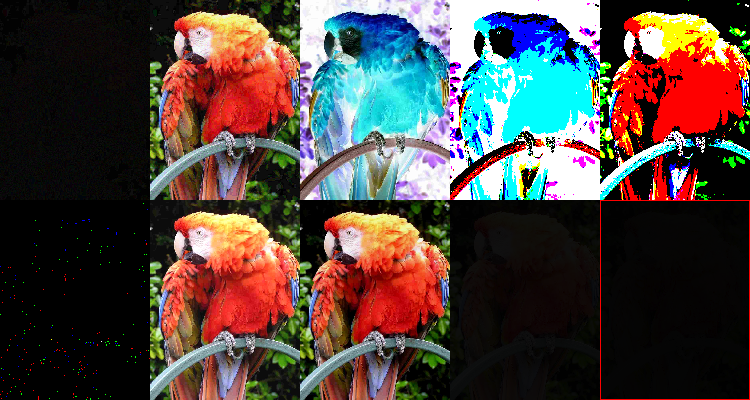
\includegraphics[width=300pt]{media/check-only-example-output}

\subsubsection{UnaryOp-pipes}
TODO: specialize UnaryOpPipe::apply(src) function to use (different from the default impl. form UnaryOp) the last pipe image.

\codefile{unary-op-pipe-example.cpp}{Example for usage of the UnaryOpPipe class}

\subsection{Binary Operations\label{subsec:binary-ops}}
In contrast to unary operations, binary operations (base class \iclclassref{Filter}{BinaryOp} implement a 2-1 input/output relationship. Binary operations are e.g. a pixel-wise addition and multiplication of images or even a proximity measurement pixel-wise comparison of two images. The \inlinecode{BinaryOp} class uses another signature for its \inlinecode{apply}-function:

\displaycode{void apply(const ImgBase *operand1, const ImgBase *operand2, ImgBase **dst)}

As you can see, the only difference to the \inlinecode{UnaryOp}'s interface is an additional second source image argument.

\subsection{Affine Operations\label{subsec:affine-ops}}

\subsection{Neighbourhood Operations\label{subsec:nbh-ops}}

\subsection{In-Place Operations\label{subsec:inplace-ops}}

\subsection{Other Operations\label{subsec:other-ops}} 
